\documentclass[12pt]{jarticle}
\usepackage[dvipdfm]{graphicx}
\begin{document}
\begin{center}
    {\Huge \underline{和とりっぷ}}

    〜桜咲く 京都 奈良の旅〜
\end{center}
\section{ホーム}
\subsection{目的}
いつも忙しくあれこれ考えすぎて、自然の美しさを忘れていませんか?
春の訪れを五感で感じ、日々の疲れを癒しましょう。
\subsection{概要}

東京を出発し京都・奈良を周る旅です。
一泊二日で短い休暇の間でもご参加いただけます。
春、桜満開の京都・奈良の寺社仏閣をめぐり、歴史と自然の調和を味わいます。
各地で記念撮影を行い、アルバムにまとめて後日販売致します。

\clearpage
\begin{center}
    {\Huge \underline{和とりっぷ}}

    〜桜咲く 京都 奈良の旅〜
\end{center}
\section{日程}
\subsection{1日目}
1日目は京都をめぐります。
東京駅を出発し新幹線で京都駅へ移動。
嵐山、金閣寺を昼のうちにまわり、夜の清水寺に繰り出します。
\begin{figure}[h]
    \begin{center}
        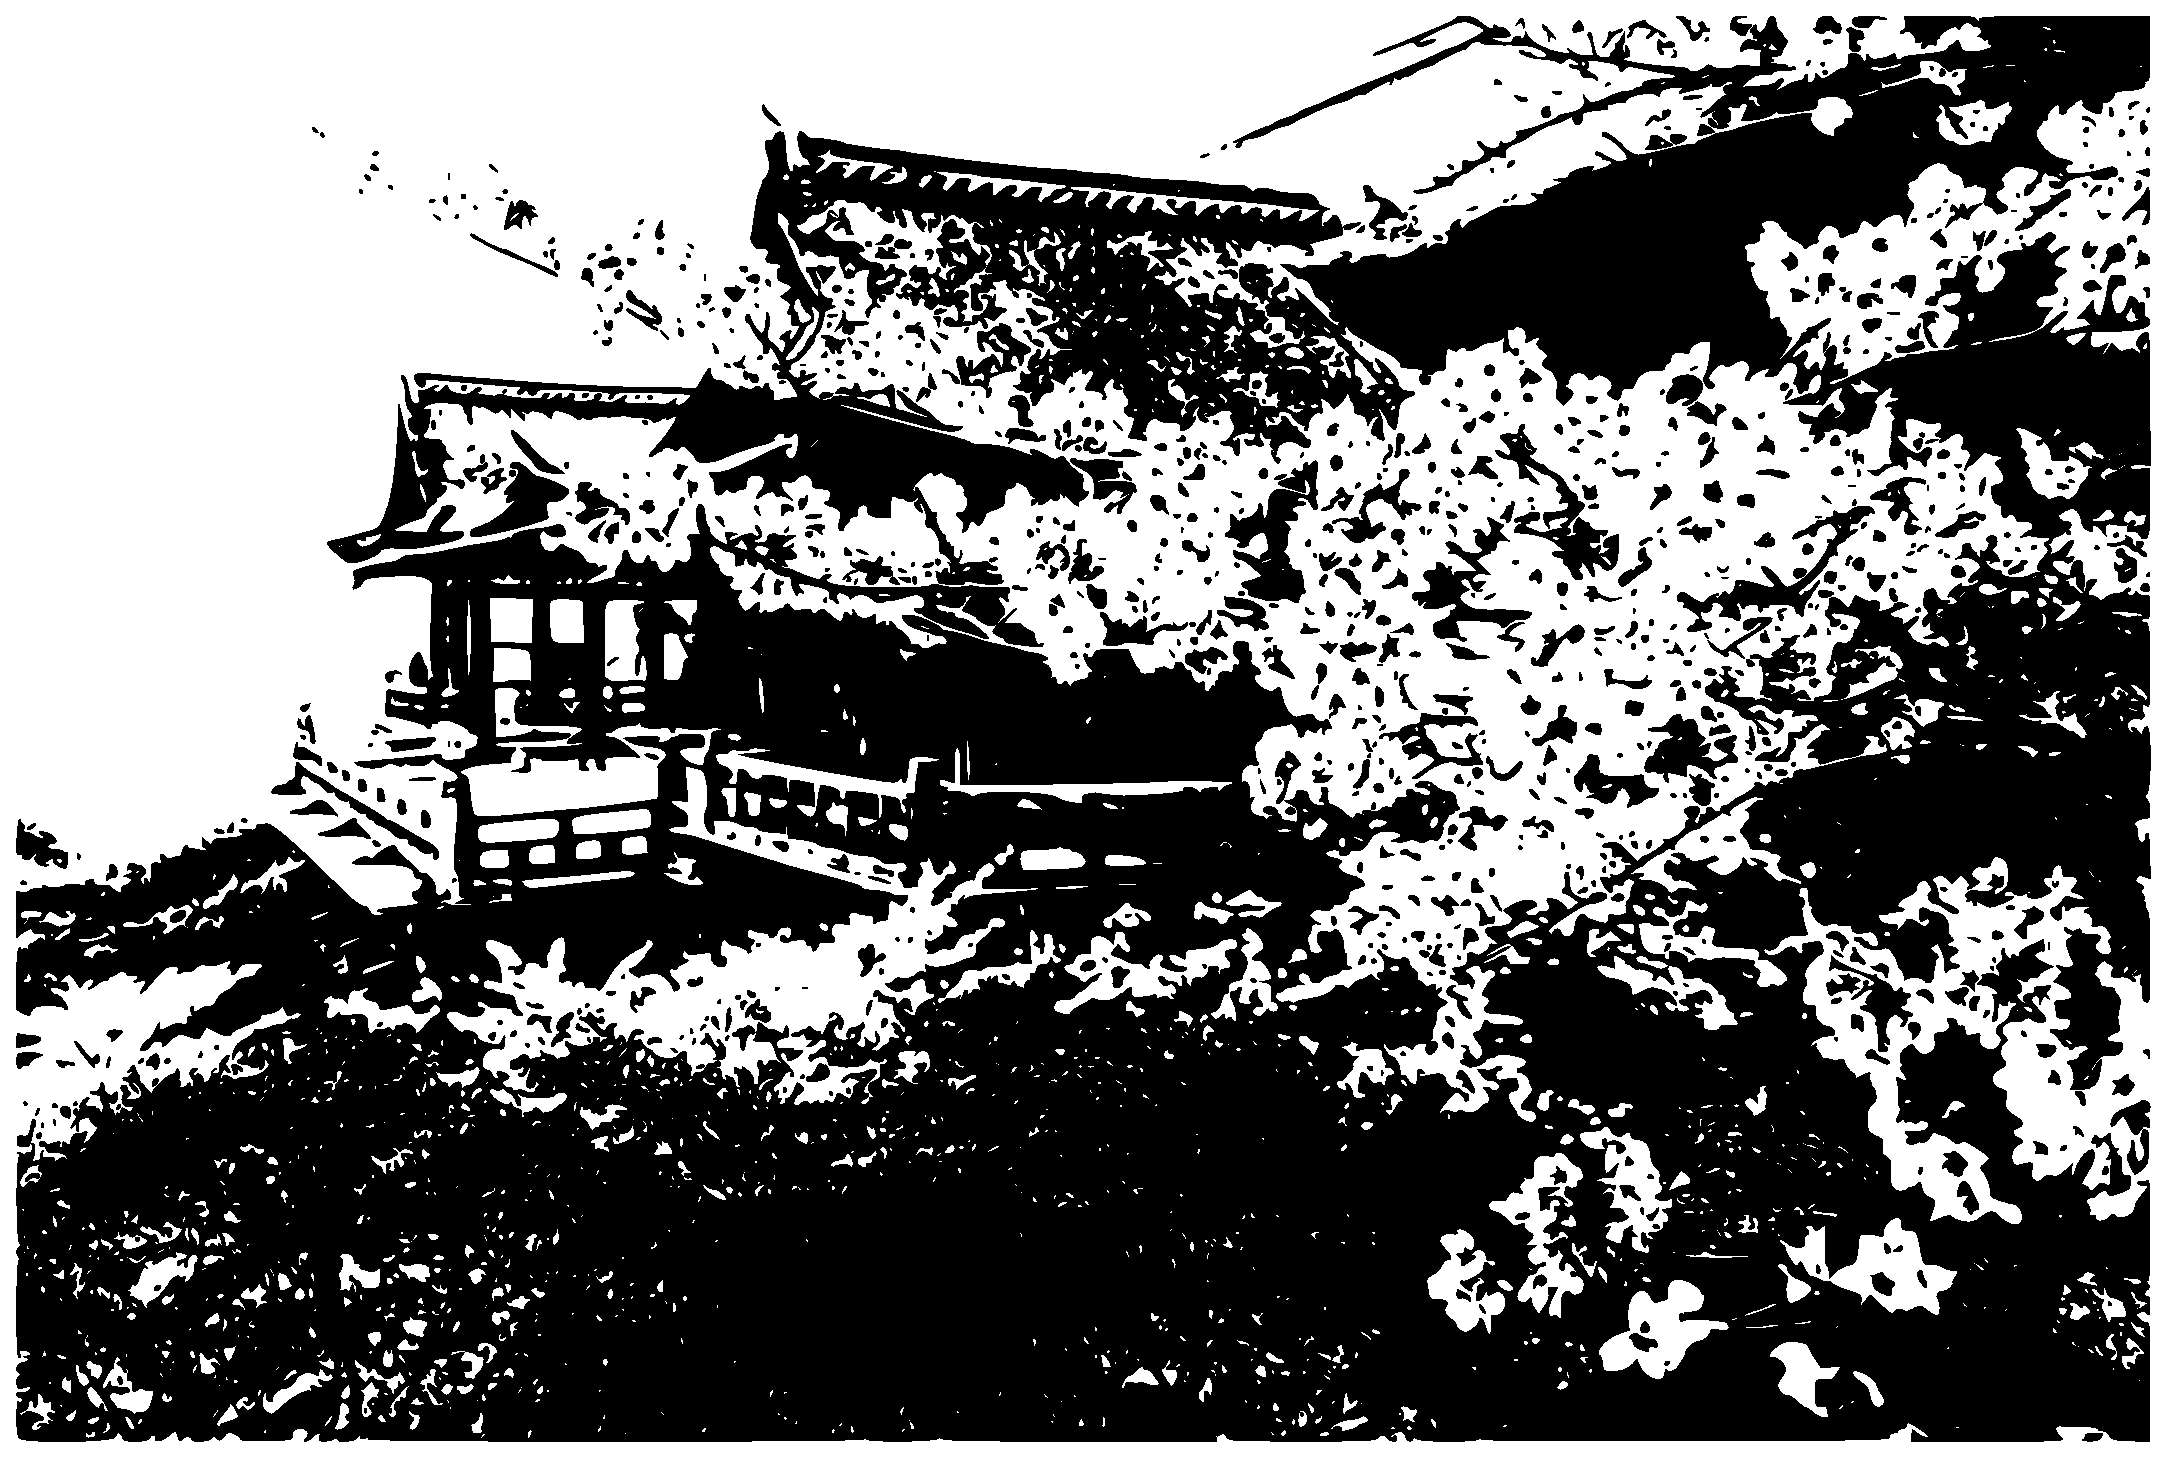
\includegraphics[height=3cm, width=5cm]{kiyomizu.eps}
    \end{center}
\caption{清水寺 (引用:https://www.kyoto-sakura.net/)}
\end{figure}

\subsection{2日目}
2日目は奈良をめぐります。 奈良に移動後、薬師寺を見たあとは奈良公園で鹿とたわむれます。 旅の最後には法隆寺・五重塔を眺めて、東京駅へと帰ります。
\begin{figure}[h]
    \begin{center}
        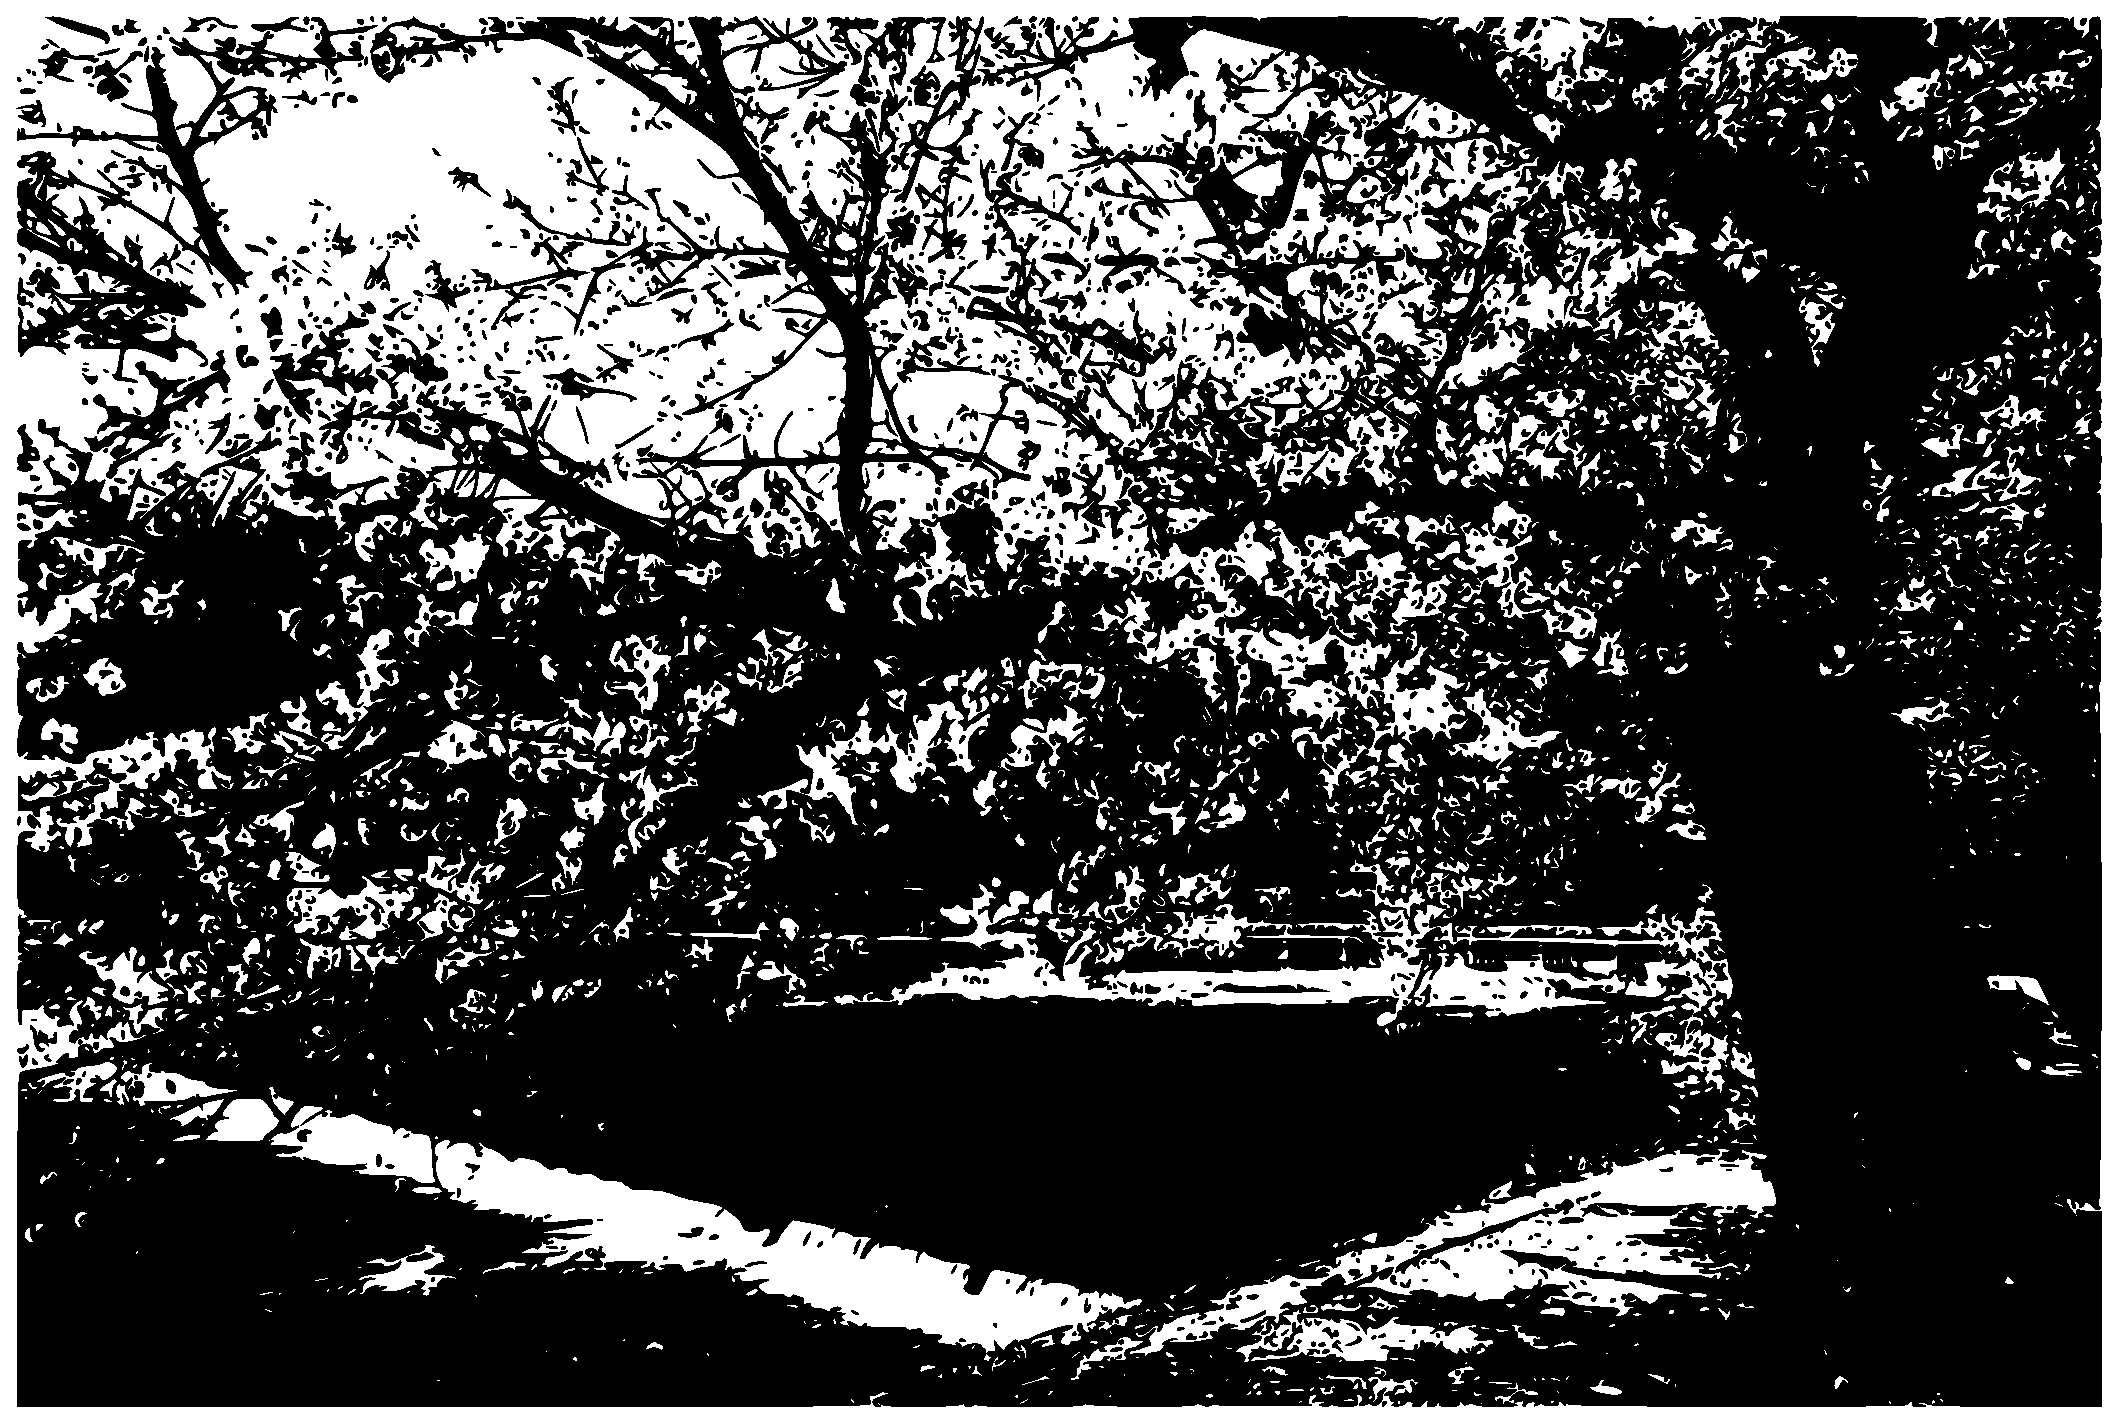
\includegraphics[height=3cm, width=5cm]{arashiyama.eps}
    \end{center}
\caption{嵐山 (引用:https://www.kyoto-sakura.net/)}
\end{figure}

\clearpage
\begin{center}
    {\Huge \underline{和とりっぷ}}

    〜桜咲く 京都 奈良の旅〜
\end{center}
\section{宿泊施設}
{\large \textbf{三木半旅館}}

address: 〒604-8072 京都市中京区六角麩屋町角 \\


長い歴史をもちながらも綺麗な内装のお宿です。
京都観光にぴったりの位置にあり快適な旅の拠点となります。
\begin{figure}[h]
    \begin{center}
        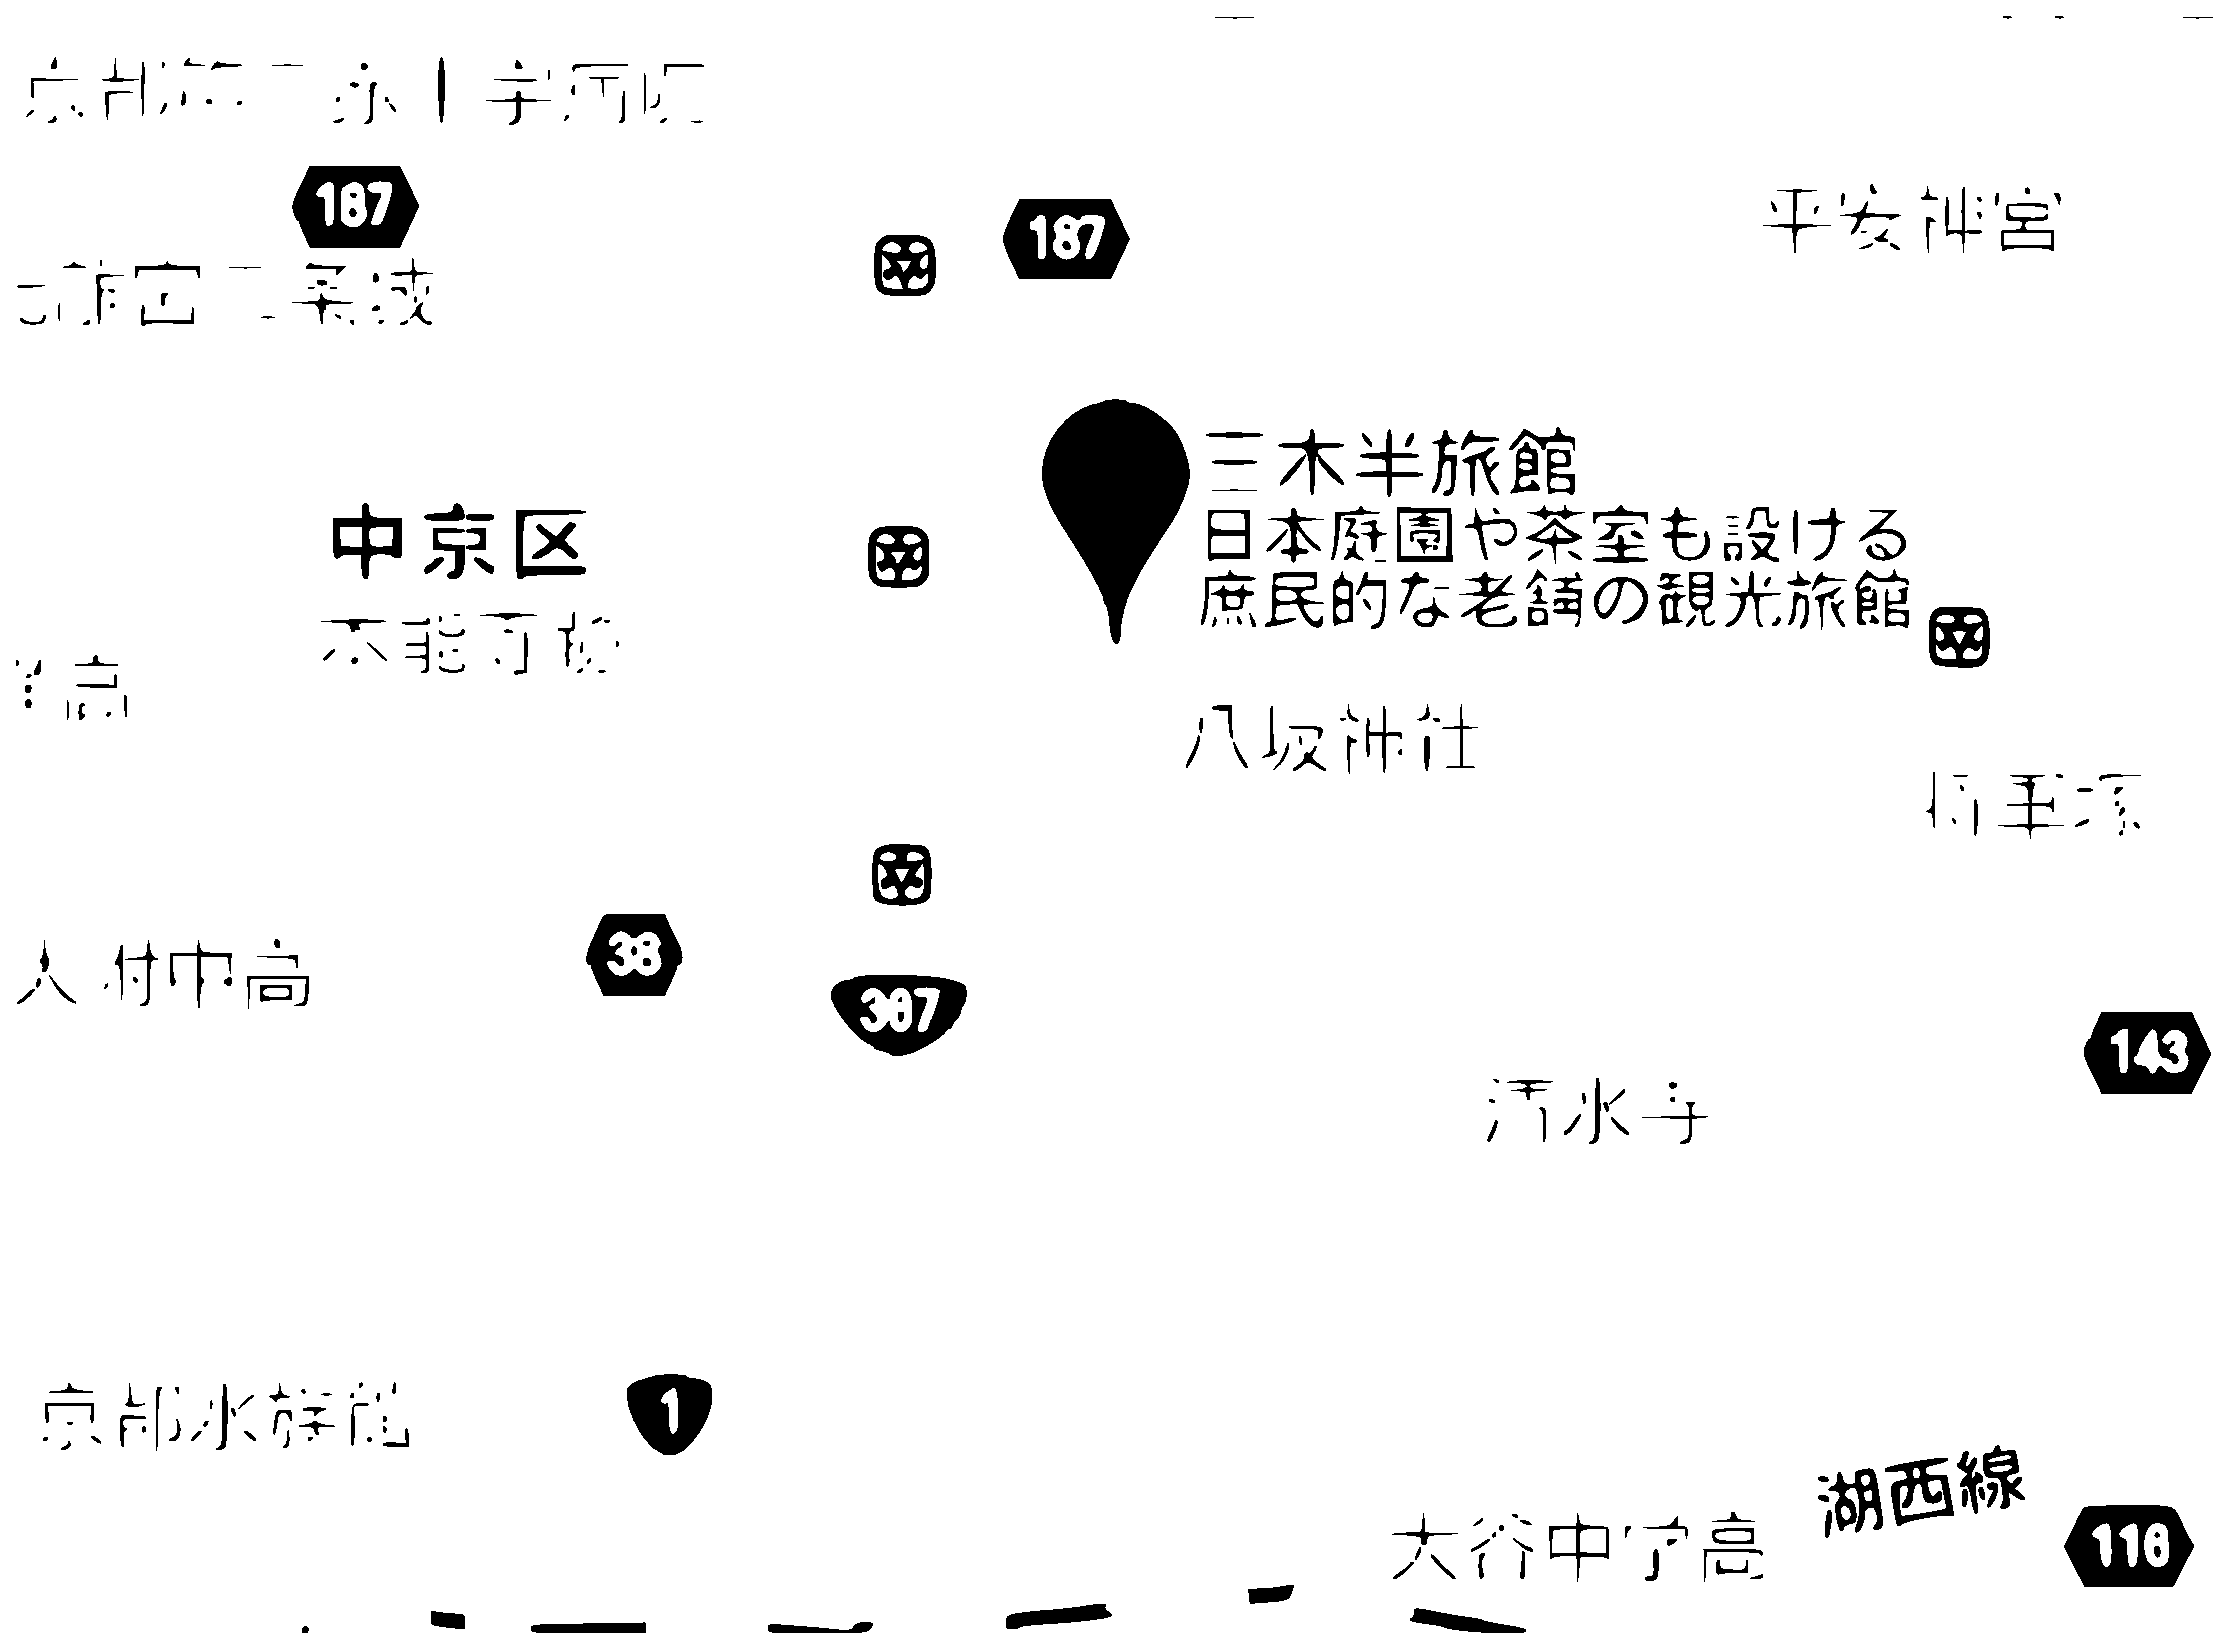
\includegraphics[height=6cm, width=10cm]{map.eps}
    \end{center}
\end{figure}

\clearpage
\begin{center}
    {\Huge \underline{和とりっぷ}}

    〜桜咲く 京都 奈良の旅〜
\end{center}
\section{タイムスケジュール}
\subsection{1日目} 
6:30 東京駅 銀の鈴周辺 集合

7:00 新幹線(ひかり) 発車

9:36 京都駅 到着

10:20 嵐山 到着

12:20 嵐山 出発

12:50 金閣寺 到着

13:30 金閣寺 出発

14:00 清水寺 到着

15:00 清水寺 出発

17:30 旅館 到着

\subsection{2日目}
7:30 旅館 出発

8:40 薬師寺 到着

9:40 薬師寺 出発

10:20 奈良公園 到着

12:30 奈良公園 出発

13:20 法隆寺 到着

15:00 法隆寺 出発

17:00 京都駅 到着

17:40 新幹線(ひかり) 発車

20:11 東京駅 到着

20:30 解散

\clearpage
\begin{center}
    {\Huge \underline{和とりっぷ}}

    〜桜咲く 京都 奈良の旅〜
\end{center}
\section{費用}
\subsection{宿泊費(二食付き)} 
30,000円
\subsection{交通費(新幹線、在来線含む)} 
30,000円
\subsection{諸費用} 
10,000円\\


{\footnotesize * 1日目、2日目の昼食時は自由行動となるため昼食費用は別途ご用意ください。}
\end{document} 